\documentclass{article}
\usepackage{amsmath}
\usepackage{graphicx}
\title{CTA200 2020 Computing project Part 1}
\author{By: Samantha Hassal}
\date{}
\begin{document}

\begin{figure}
  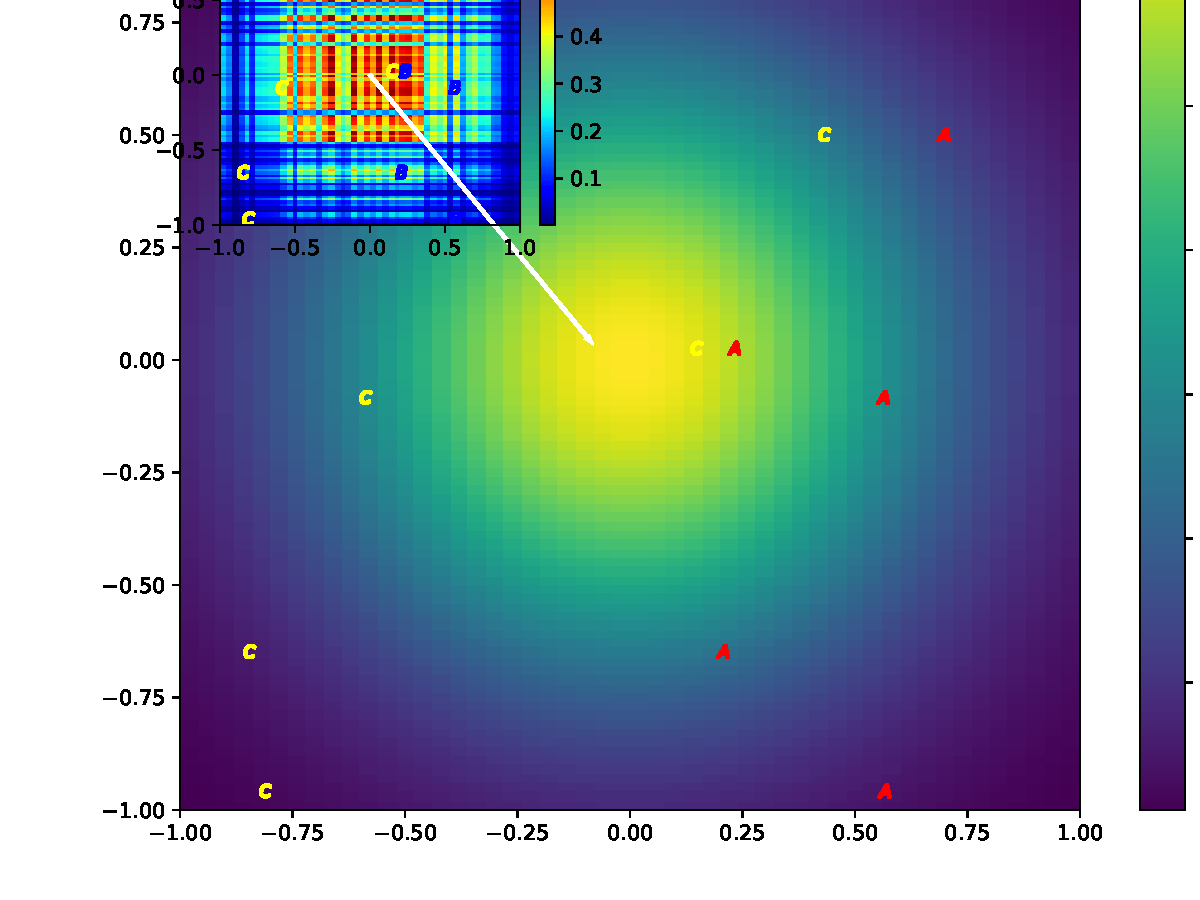
\includegraphics[width=\linewidth]{SamanthaHassal-graphing-demo.pdf}
  \caption{An image of a 2D Gaussian distribution $P(x,y)=\frac{2.0 e^{- 2.0 x^{2} - 2.0 y^{2}}}{\pi}$. Such a distribution requires a mean vector (in this case, this vector is zero) and a covariance matrix. If I chose to build a generic function that creates a 2D Gaussian, I would use the mean vector, covariance matrix, and integers that represent array sizes. The inset of theis graph uses the jet colour map, while the main axis uses the viridis colour map. I would use the viridis colour map over the jet colour map becuase not only does it translate to grayscale easier, but colourblind people will have an easier time reading it.}
  \label{fig:2d-gaussian}
\end{figure}

\end{document}
